\documentclass{article}

\usepackage[utf8]{inputenc}

\usepackage{siunitx}		% si units
\usepackage{graphicx}	% images
\usepackage{amsmath, amssymb, amsthm}
\usepackage{textcomp}	% degree symbol

\usepackage{booktabs}	% better tables

\usepackage{listings}		% code listings with highlighting
\usepackage{courier}		% change listings to courier font


\lstset{basicstyle=\footnotesize\ttfamily,breaklines=true}
\lstset{framextopmargin=50pt,frame=bottomline}
\lstset{showstringspaces=false}

\graphicspath{ {images/} }


\title{Structure and oxygen affinity of myoglobin: an MD study}
\author{Jason \textsc{Weinzierl} \\
\textit{Department of Physics and Astronomy,} \\
\textit{University of Missouri, Columbia, Missouri 65211-7010, USA}}
\date{(\today)}

\begin{document}

\maketitle

\begin{figure}[h]
	\centering
	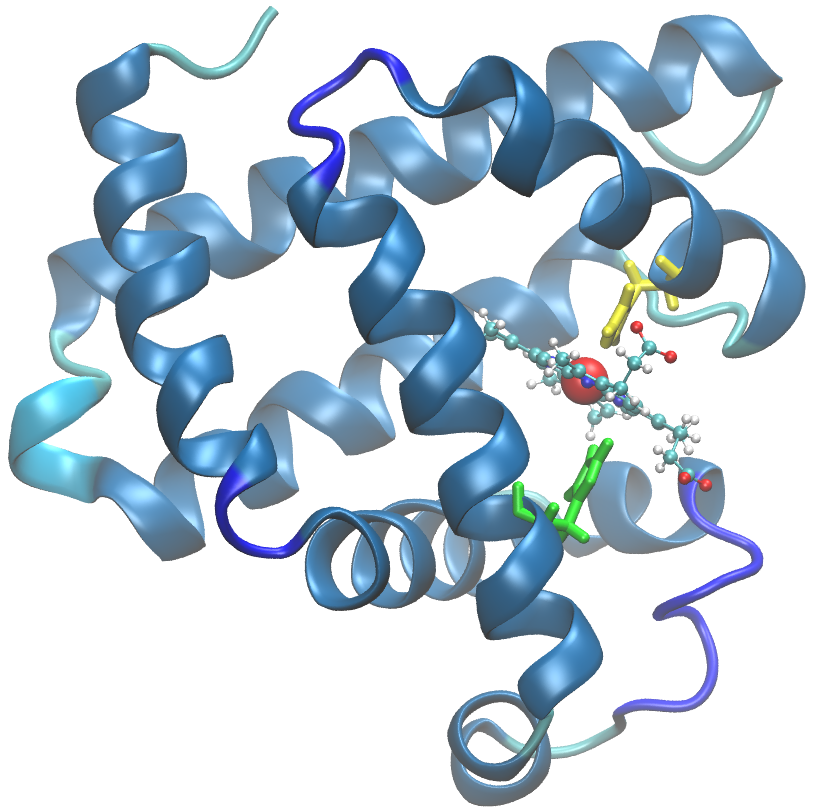
\includegraphics{myoglobin.png}
\end{figure}

\begin{abstract}
Using molecular dynamics simulations, we investigate the structure and oxygen affinity of the small protein \textbf{myoglobin}.  We find that the protein's structure is generally conserved across species.  We also demonstrate with MD simulations that oxygen enters myoglobin through cavities which open and close with thermal fluctuations.  Finally, we show that myoglobin resists fatal binding with carbon monoxide by restricting the Fe--C--O or Fe--O--O binding angles at the heme group.
\end{abstract}

\section{Introduction}

Myoglobin is a small protein found in the muscle of vertebrates.  Myoglobin binds oxygen reversibly and is similar to hemoglobin, the oxygen-carrier found in blood.  Myoglobin acts a pigment in muscle tissue, causing it to appear red.  The function of this 154-residue protein is thought to be oxygen storage.  In a cleft of myoglobin is a heme group with an atom of iron in the center (Figure~\ref{fig:heme}).

In this project, we study the general structure of myoglobin and how it fulfills its role in reversibly binding with oxygen.  We look at oxygen pathways to the cleft containing the heme.  We also look at how myoglobin resists binding carbon monoxide, which is irreversible and catastrophic.

\begin{figure}
	\centering
	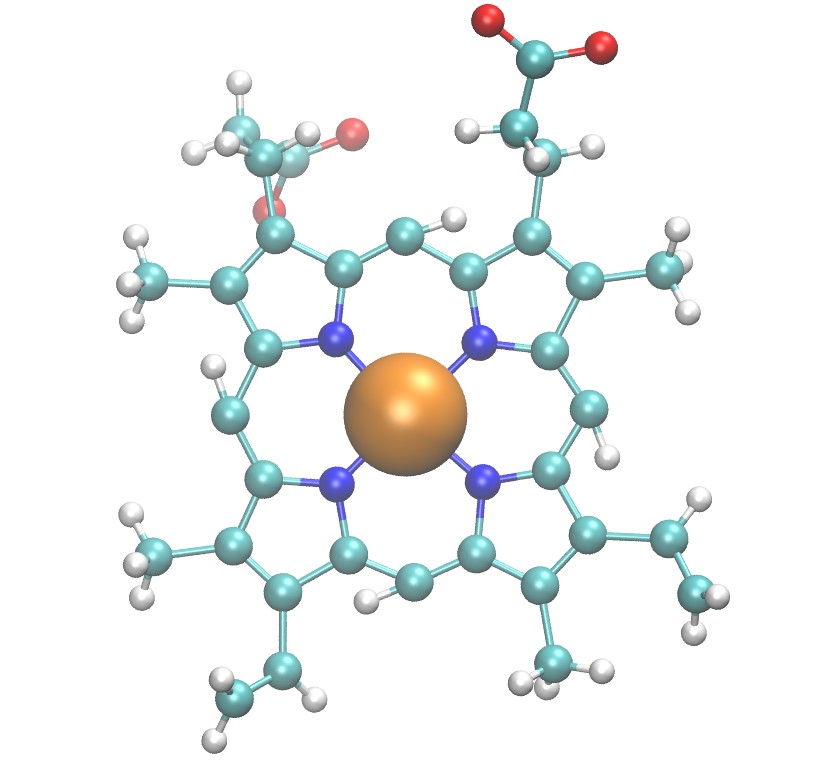
\includegraphics[width=0.5\textwidth]{heme.png}
        \caption{The heme group, featuring the orange iron atom at the center, supported by four N atoms (not shown: the supporting proxiaml histidine).}
	\label{fig:heme}
\end{figure}



\section{Methods}

\subsection{Visualizing structure}

We first use VMD to display the demonstrate Myoglobin's structure: eight alpha-helices of the protein, the heme group with an iron in the center, the \textbf{proximal histidine} anchoring the heme, and the distal histidine, which will come into play when investigating binding angles.

For presenting the ubiquity of myoglobin, we obtain from the protein databank:

\begin{itemize}
	\item \lstinline|aplysia-1MBA.pdb|
	\item \lstinline|horse-1WLA.pdb|
	\item \lstinline|seal-1MBS.psb|
	\item \lstinline|tuna-1MYT.pdb|
	\item \lstinline|turtle-1LHS.pdb|
	\item \lstinline|whale-1MBC.pdb|
\end{itemize}

After importing the crystal structures, we align the proteins using the VMD Extension Multiseq \cite{multiseq}.

\begin{figure}
  \centering
  \begin{minipage}{0.4\textwidth}
    \centering
    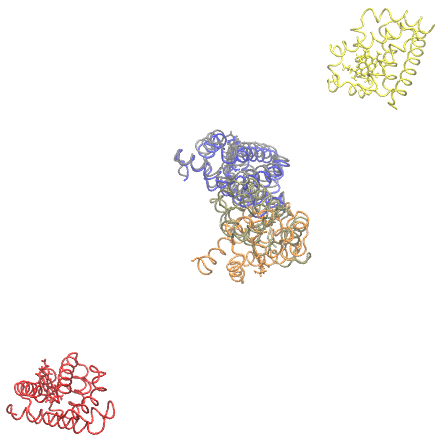
\includegraphics[width=\linewidth]{loadalign.png}
    \caption{Initial visualization window, before aligning proteins.}
    \label{fig:loadalign}
  \end{minipage}
  \hfill
  \begin{minipage}{0.5\textwidth}
    \centering
    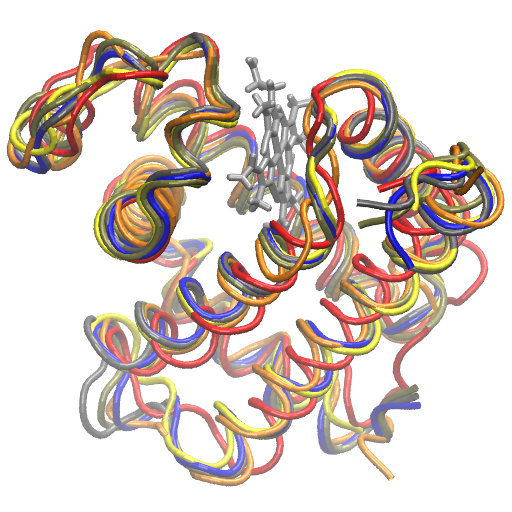
\includegraphics[width=\linewidth]{multiseq.png}
    \caption{Aligned proteins. Whale in blue, aplysia in red, horse in grey, seal in orange, tuna in yellow, turtle in bronze.}
    \label{fig:multiseq}
  \end{minipage}
\end{figure}

We expect from the literature that the \textit{Aplysia limacina} myoglobin is least conserved from the others \cite{tutorial}.

\subsection{Demonstrating oxygen access}

Myoglobin is tightly packed with side groups to protect the heme from oxidizing or binding with other unwanted molecules.  This also shields the heme from oxygen.  Yet, we know that oxygen must reach the heme group somehow.  From a static picture, we demonstrate that there are no `oxygen channels'.  But we should find, over time, that cavities arise due to thermal fluctuations of the residues.  The probabilistic motion spreads cavities throughout and eventually allows O$_2$ to reach the heme.  This happens on a timescale from nanoseconds to microseconds.

The case study files provided by UIUC \cite{tutorial} give a glimpse into the interior of myoglobin over time.  To compare with the image (Figure~\ref{fig:uiuc}), we have a simulated myoglobin trajectory for \SI{200}{\pico\second} in water.  We display the RMSD per residue of the protein and compare the results to the UIUC data in our Results section.

\subsection{Heme simulation}

Finally, we show how myoglobin resists binding irreversibly to carbon monoxide.  On the oxygen-binding side of the heme, the \textbf{distal histidine} is believed to enforce the binding angle of the ligand to the heme e.g. the Fe--O--O or Fe--C--O angles.  We define \textbf{binding angle} as the Fe--O--O or Fe--C--O angles for oxygen or carbon monoxide molecules respectively.

% TODO: energetic cost associated with enforcing a shallow binding angle

% TODO: slug binding site might have different function

So if a shallow binding angle (less than 180\textdegree) is enforced in myoglobin, then we will show the desired binding angles of CO and O$_2$ to the heme, outside of the protective structure of the myoglobin protein.  Without the distal histidine interfering with binding, CO should remain nearly straight, while oxygen should have a more shallow angle with a larger RMSD.  These simulations are \SI{500}{\pico\second} in water, and we plot the angles over time, demonstrating averages and RMSD fluctuation in the angle in our Results.

\section{Results and Discussion}

\subsection{Structure and conservation across species}

Figure~\ref{fig:alpha_helices} shows the strong helix structure of myoglobin, and Figure~\ref{fig:histidines} shows the two histidines and bound oxygen on the heme.  The unbounded heme group was shown previously in Figure~\ref{fig:heme}.

\begin{figure}[!b]
	\centering
	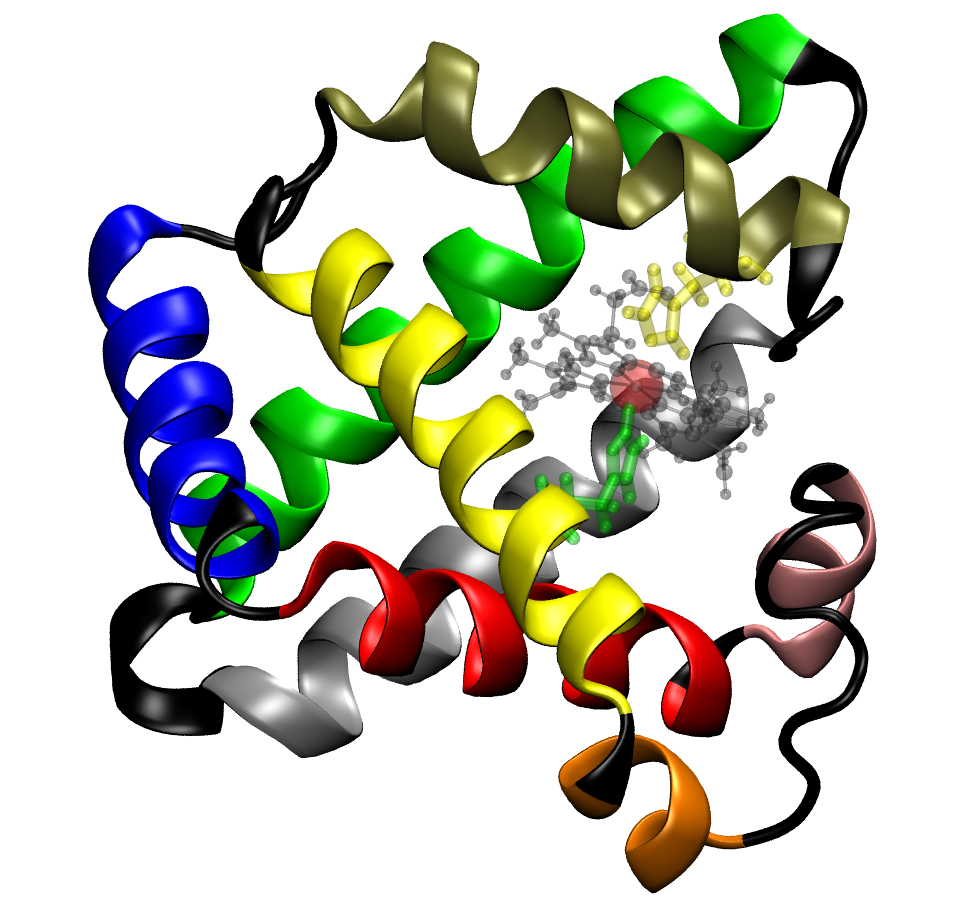
\includegraphics[width=0.5\textwidth]{alpha_helices.png}
	\caption{The eight alpha helices of whale myoglobin.  Alpha helix 1 (residues 4 to 18) is colored blue, helix 2 (21 to 35) is red, helix 3 (37 to 42) is pink, helix 4 (52 to 57) is orange, helix 5 (59 to 77) is yellow, helix 6 (82 to 96) is bronze, helix 7 (101 to 119) is silver, and helix 8 (125 to 149) is green.  The rest of the secondary structure is in black and the heme/histidines core is transparent.}
	\label{fig:alpha_helices}
\end{figure}

\begin{figure}
	\centering
	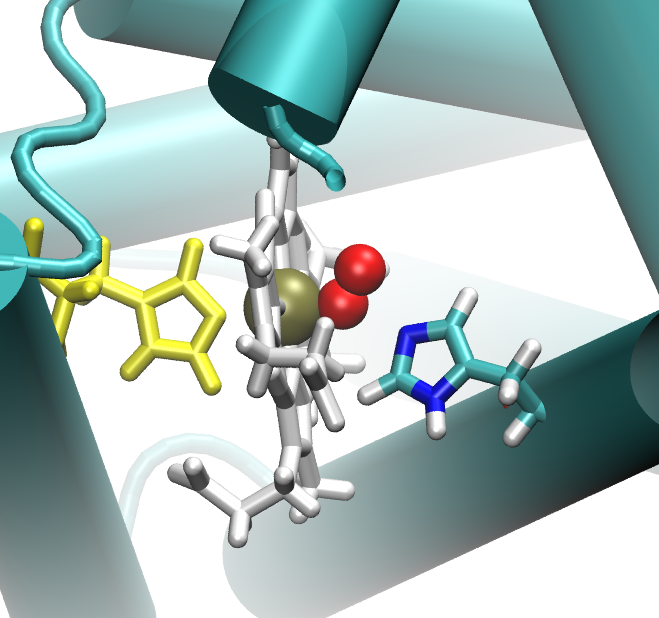
\includegraphics[width=0.5\textwidth]{histidines.png}
	\caption{the heme, colored white with a bronze fe, bound to red oxygen.  the heme is anchored to the proximal histidine, in yellow.  the distal histidine, colored by atom name, forces oxygen to bind at a shallower angle than 180\textdegree to the iron center.}
	\label{fig:histidines}
\end{figure}

Now we look at myoglobin of six species: \textit{Aplysia limacina} (mottled sea hare), \textit{Equus caballus} (horse), \textit{Phoca vitulina} (seal), \textit{Thunnus albacares} (yellowfin tuna), \textit{Caretta caretta} (sea turtle), and \textit{Physeter macrocephalus} (sperm whale).  Figure~\ref{fig:species} shows the six myoglobins overlayed.

\begin{figure}
	\centering
	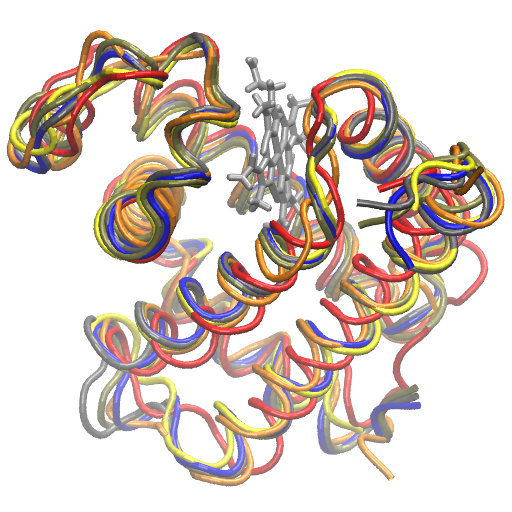
\includegraphics[width=0.5\textwidth]{multiseq.png}
        \caption{Notice that the aplysia myoglobin, colored red, has the most deviations in secondary structure from the other five species' myoglobin.  This is reasonable considering it lives wholly under water and has no need to hold its breath, which myoglobin's oxygen-storing properties would enhance in air-breathing organisms.}
	\label{fig:species}
\end{figure}


\subsection{Oxygen pathways}

From Figure~\ref{fig:uiuc}, we see that pathways for oxygen to travel through do indeed appear over time.  So while myoglobin may appear closed to oxygen, it is open when fluctuating normally.  In Figure~\ref{fig:beta}, we see that, when looking at RMSD per residue over time, the most common fluctuations happen near the heme, allowing oxygen a probabilistically shorter pathway to the heme.

\begin{figure}
  \centering
  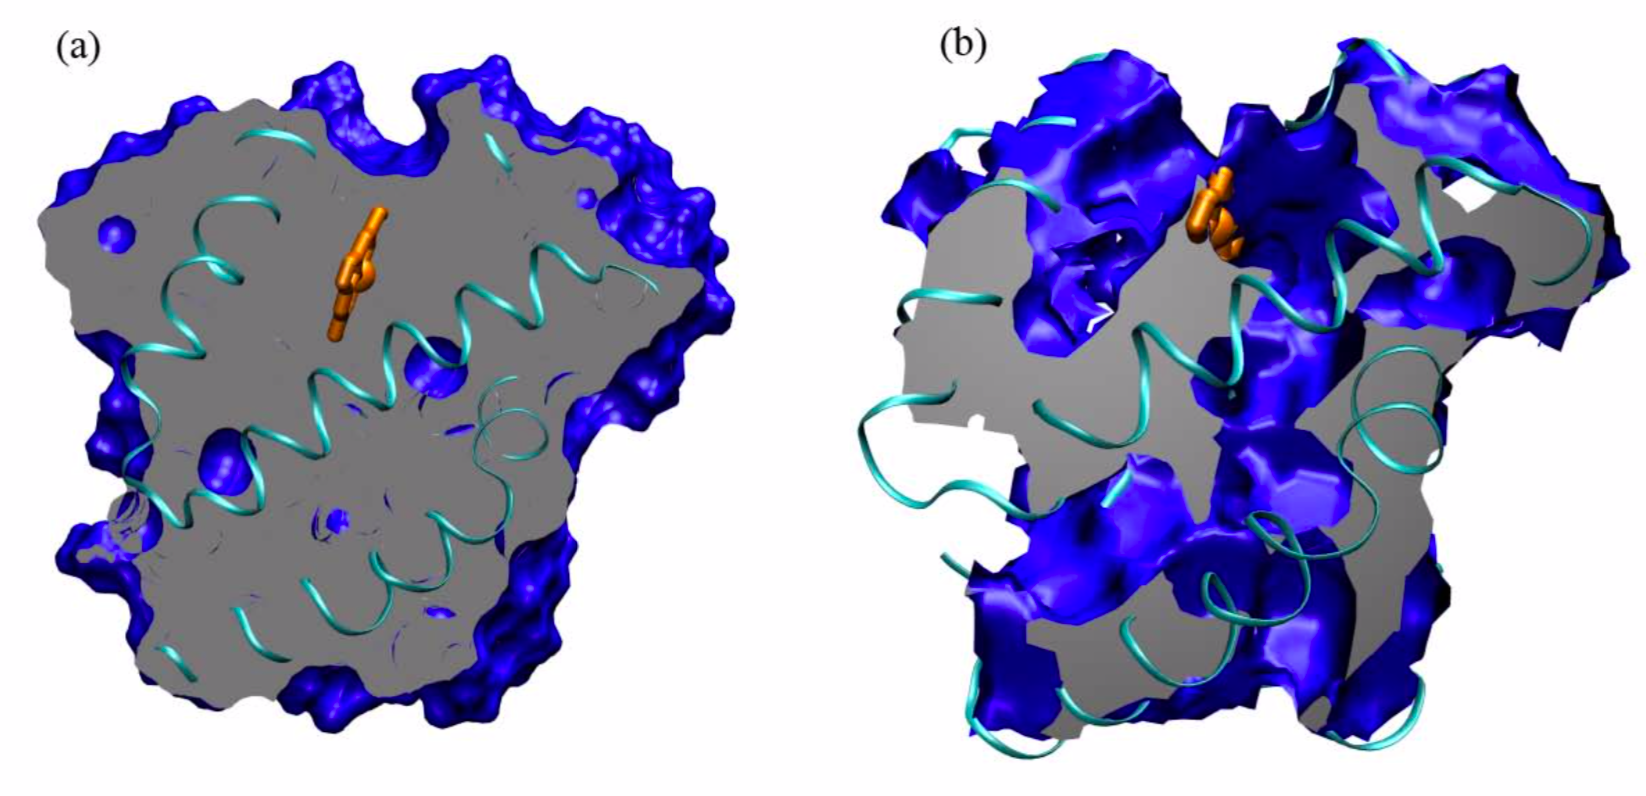
\includegraphics[width=\textwidth]{interior.png}
  \caption{The interior of myoglobin.  In the first image, the static structure shows very little accessibility to oxygen: cavities open to oxygen are in blue and inaccessible areas are in gray.  In the second image, however, cavities arise and a pathway can be seen over time due to movement of the residues. (figure from \cite{tutorial})}
  \label{fig:uiuc}
\end{figure}

\begin{figure}
  \centering
  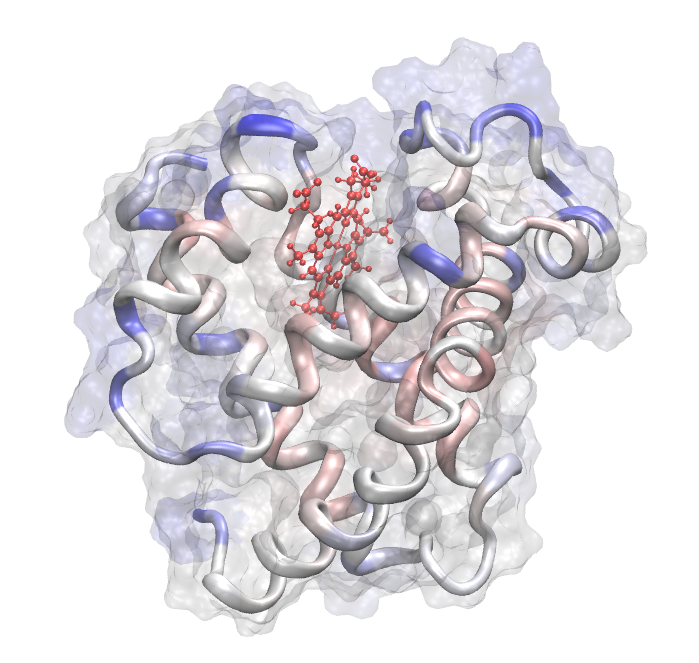
\includegraphics[width=0.5\textwidth]{beta.png}
  \caption{RMSD by residue of whale myoglobin in water for \SI{200}{\pico\second}.  Note that it lines up with the previous Figure~\ref{fig:uiuc}; the blue areas tend to fluctuate wildly, while the red stays static.  Oxygen pathways to the heme should open up in the blue areas.}
  \label{fig:beta}
\end{figure}

\subsection{Binding angles of O$_2$ and CO}

\begin{figure}
  \centering
  \begin{minipage}{0.4\textwidth}
    \centering
    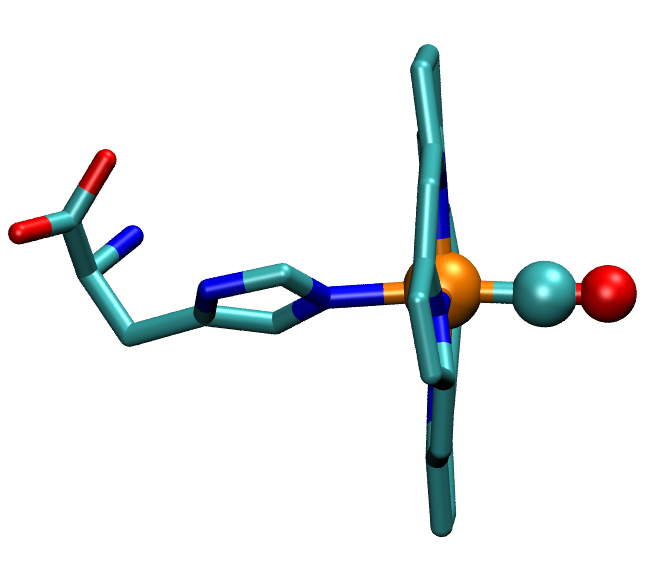
\includegraphics[width=\linewidth]{coheme.png}
    \caption{CO bound to heme in the absence of myoglobin's surrounding structure.  This is a snapshot from a \SI{500}{\pico\second} trajectory in water.  Note that it prefers a near-straight angle.}
    \label{fig:coheme}
  \end{minipage}
  \hfill
  \begin{minipage}{0.5\textwidth}
    \centering
    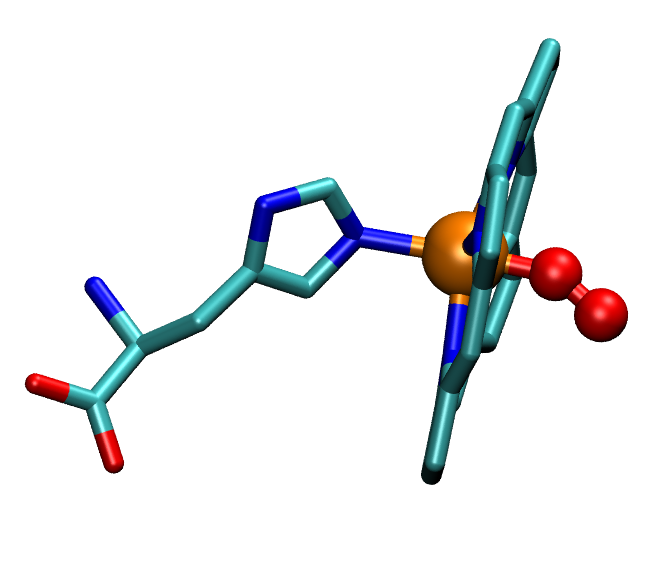
\includegraphics[width=\linewidth]{o2heme.png}
    \caption{O$_2$ bound to heme again without myoglobin forcing any binding angle.  Throughout the \SI{500}{\pico\second} trajectory, the O$_2$ molecule fluctuates its binding angle rapidly, with straight preference like CO.}
    \label{fig:o2heme}
  \end{minipage}
\end{figure}

In Figures \ref{fig:coheme} and \ref{fig:o2heme}, we see a snapshot from a simulation of carbon monoxide and oxygen binding the heme group.  Throughout the trajectory, CO prefers a straight angle while O$_2$ fluctuates wildly with no preferred angle.  These simulations take place outside of myoglobin.

\begin{figure}
  \centering
  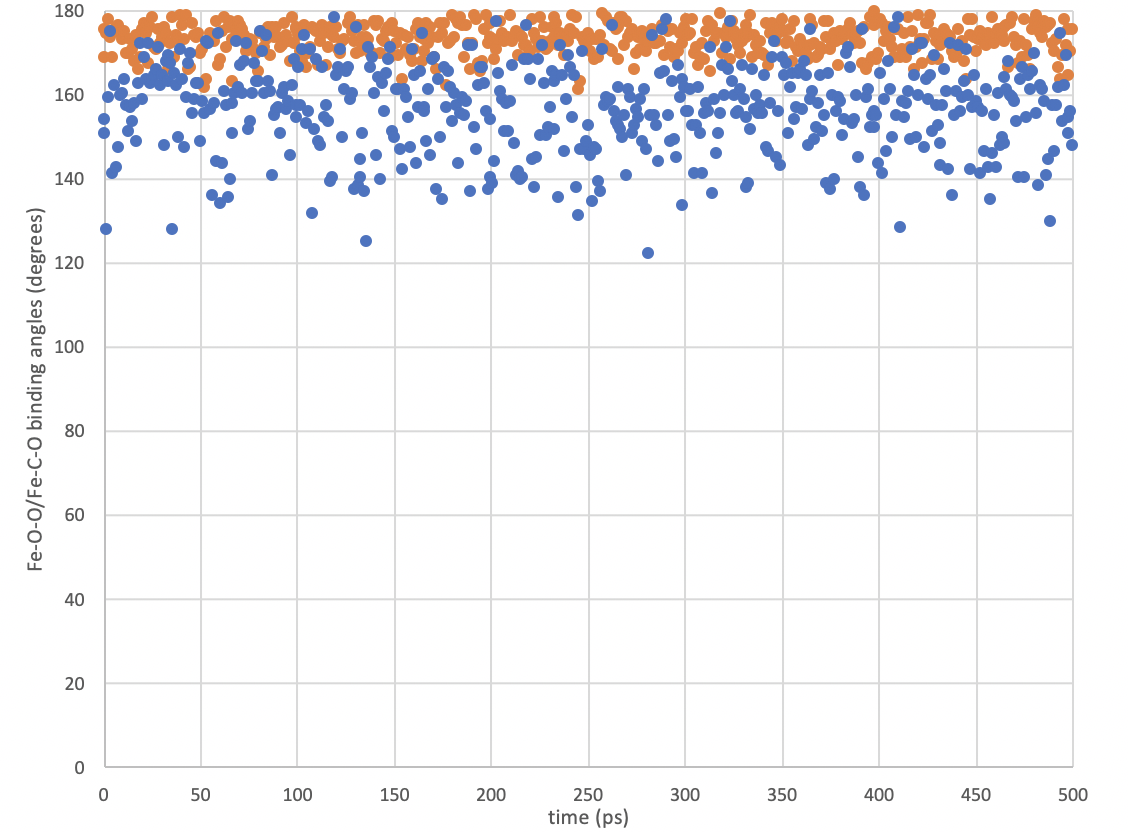
\includegraphics[width=\textwidth]{angles.png}
  \caption{Plots of Fe--O--O angle (in blue) and Fe--C--O (in orange) angle over time.  The Fe--O--O angle has a higher fluctuation and lower average angle than that of Fe--C--O.}
  \label{fig:time}
\end{figure}

Figure~\ref{fig:time} shows the binding angles (Fe--O--O or Fe--C--O angles) over the time of the simulation.

So, when inside myoglobin, if the distal histidine forces incoming molecules to bind at a shallow angle to the heme as is hypothesized \cite{tutorial}, then this indicates that CO will be very unlikely to bind because it \emph{prefers a straighter angle}.  This is how myoglobin resists permanently binding CO---the distal histidine should make CO's desired angle difficult to reach, while O$_2$ binds easily at the shallow angle.

\section{Conclusion}

We've displayed the structures of myoglobin across species, simulated how oxygen's entry is made easier by myoglobin's structure, and showed how it resists carbon monoxide binding.


\begin{thebibliography}{9}
\bibitem{tutorial}
	Anton Arkhipov, Rosemary Braun, and Ying Yin,
	\textit{Case Study: Myoglobin},
	University of Illinois at Urbana-Champaign, Illinois,
	21 February 2008.
	
\bibitem{vmd}
	Humphrey, W., Dalke, A. and Schulten, K., `VMD - Visual
	Molecular Dynamics', J. Molec. Graphics 1996, 14.1, 33-38.

\bibitem{secondary}
	Frishman,D \& Argos,P. (1995) Knowledge-based secondary structure
	assignment. Proteins: structure, function and genetics, 23, 566-579.

\bibitem{multiseq}
        Elijah Roberts, John Eargle, Dan Wright, and Zaida Luthey-Schulten.
        MultiSeq: Unifying sequence and structure data for evolutionary analysis.
        \textbf{BMC Bioinformatics, 2006, 7:382}.

\end{thebibliography}

\vspace{\fill}

\centering{Prepared with \LaTeX.}


\end{document}
